\chapter{Ergebnisse}
\label{ch:chapter04}
In diesem Kapitel werden die Ergebnisse der Messungen für die verschiedenen Scheduler vorgestellt, 
miteinander verglichen und im Anschluss diskutiert.
Im Anhang befinden sich alle Grafiken zu den Messungen in nach Scheduling-Algorithmus geordneter Reihenfolge.
\begin{sloppypar}

\vspace{7.56mm}
\noindent Die Ergebnisse werden in vier Abschnitten präsentiert:
\begin{itemize}
    \item Zunächst werden die Ergebnisse des alten Schedulers als Referenz vorgestellt, um die Performance der neuen Scheduler bewerten zu können.
    \item Anschließend werden die Ergebnisse des FIFO-Schedulers vorgestellt und mit der Referenz verglichen, um die Auswirkungen der Einführung eines taskbasierten Schedulers zu bewerten.
    \item Danach werden die Ergebnisse des SSTF-Schedulers vorgestellt und mit dem FIFO-Scheduler verglichen, um die Auswirkungen der Priorisierung von Tasks mit kürzerer erwarteter Ausführungszeit zu bewerten.
    \item Schließlich werden die Ergebnisse des Work-Stealing-Schedulers mit SSTF-Priorisierung vorgestellt und mit dem SSTF-Scheduler verglichen, um die Auswirkungen der Kombination von Work-Stealing mit einer Priorisierungsstrategie zu bewerten.
    \end{itemize}
Die Algorithmen bauen aufeinander auf, sodass die Ergebnisse des vorherigen Schedulers jeweils als Baseline für die Bewertung des nachfolgenden Schedulers herangezogen werden.
Nach jeder Vorstellung der Ergebnisse eines Schedulers erfolgt eine Diskussion der Ergebnisse. Am Ende des Kapitels werden die Ergebnisse aller Scheduler miteinander verglichen und diskutiert. 


\section{rekursiv-synchroner, objektbasierter Scheduler (Referenz)}

Der nicht optimierte Scanner wurde als Referenz für die Messungen mit dem neuen Scheduler verwendet.
In der Tabelle \ref{tab:old-scheduler-uebersicht} sind die Mittelwerte der Laufzeit, CPU-Auslastung, 
RAM-Auslastung (Mittel und Max) sowie der Variationskoeffizient der Laufzeit für die Messungen 
mit dem alten Scheduler aufgelistet.
Die internenen Metriken wurden bei diesem nicht erhoben, um die Performance des alten Schedulers nicht zu beeinträchtigen.

\begin{table}[H]
\caption{Übersicht der Ergebnisse des alten Schedulers (Mittelwerte $\pm$ Standardabweichung aus $n=20$ Läufen)}
\label{tab:old-scheduler-uebersicht}
\centering
\begingroup
\setlength{\tabcolsep}{4pt}
\resizebox{\textwidth}{!}{%
\begin{tabular}{@{}lllllll@{}}
\toprule
Threads & OS & Runtime [s] & CPU [\%] & RAM Mittel [MB] & RAM Max [MB] & Runtime CV [\%] \\
\midrule
1 & Linux   & 643 $\pm$ 3.89 & 24.0 $\pm$ 0.00 & 1069 $\pm$ 17.8 & 1670 & 0.60 \\
4 & Linux   & 266 $\pm$ 2.61 & 55.0 $\pm$ 0.32 & 1492 $\pm$ 22.5 & 2612 & 0.98 \\
10 & Linux  & 221 $\pm$ 3.07 & 63.0 $\pm$ 0.74 & 1866 $\pm$ 36.9 & 3374 & 1.39 \\
1 & Windows & 2514 $\pm$ 8.57 & 21.0 $\pm$ 0. & 1350 $\pm$ 2.15 & 5937 & 0.34 \\
4 & Windows & 1214 $\pm$ 27.0 & 46.6 $\pm$ 0.80 & 2019 $\pm$ 50.5 & 7306 & 2.22 \\
10 & Windows & 826 $\pm$ 20.5 & 68.5 $\pm$ 1.96 & 2879 $\pm$ 281 & 12190 & 2.49 \\
\bottomrule
\end{tabular}%
}
\endgroup
\end{table}

\begin{figure}[H]
\centering
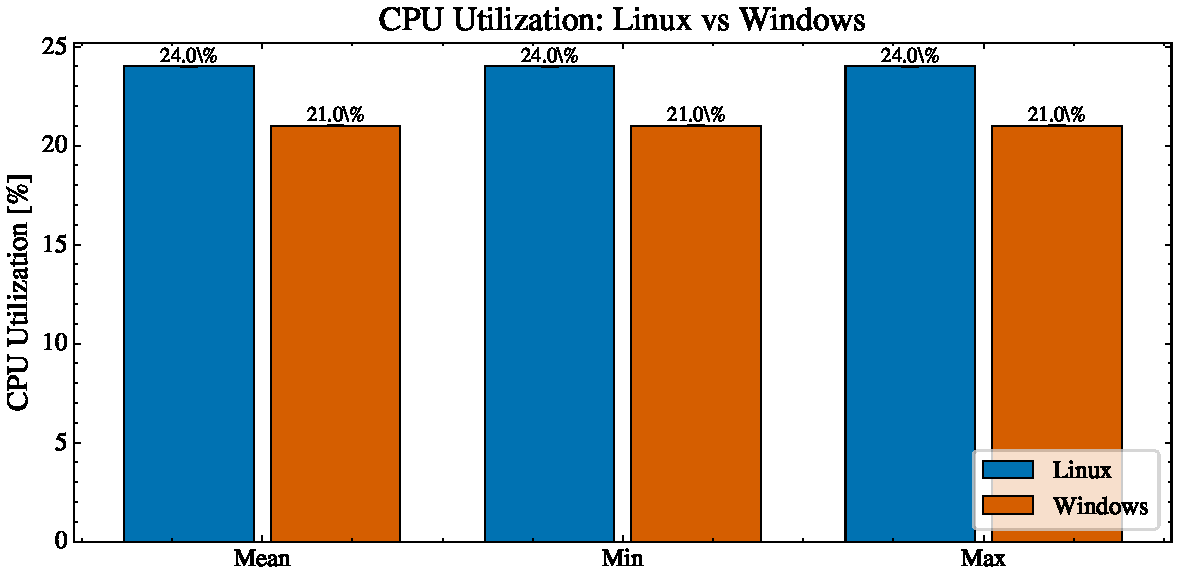
\includegraphics[width=\textwidth]{Messungen/OLD_1T/cpu_bars_combined.pdf}
\caption{Referenz, ein Thread: CPU-Utilization}
\label{fig:4ref-1t-cpu}
\end{figure}

Für die Bewertung der Stabilität des Testsystems ist zunächst die CPU-Auslastung maßgeblich. Bei der Ausführung mit einem Thread liegt diese konstant bei ca. 24\% (Linux) bzw. 21\% (Windows), wie in Abbildung \ref{fig:4ref-1t-cpu} dargestellt. Dies deutet auf ein stabiles System mit geringen Hintergrundinterferenzen hin. 
Während die CPU-Auslastung bei vier Threads noch relativ stabil bleibt (54\%--56\% bei Linux, 45\%--47\% bei Windows), ist bei zehn Threads eine deutlich größere Varianz zu beobachten (siehe Abb. \ref{fig:4ref-10t-cpu}). 
Diese Instabilität korreliert mit den Laufzeiten, die bei zunehmender Thread-Anzahl variabler werden. Dies verdeutlicht der Anstieg des Variationskoeffizienten (\textit{Runtime CV}) in Tabelle \ref{tab:old-scheduler-uebersicht} 
sowie der visuelle Vergleich der Abbildungen \ref{fig:ref-1t-runtime}, \ref{fig:ref-4t-runtime} und \ref{fig:ref-10t-runtime}.

\begin{figure}[H]
\centering
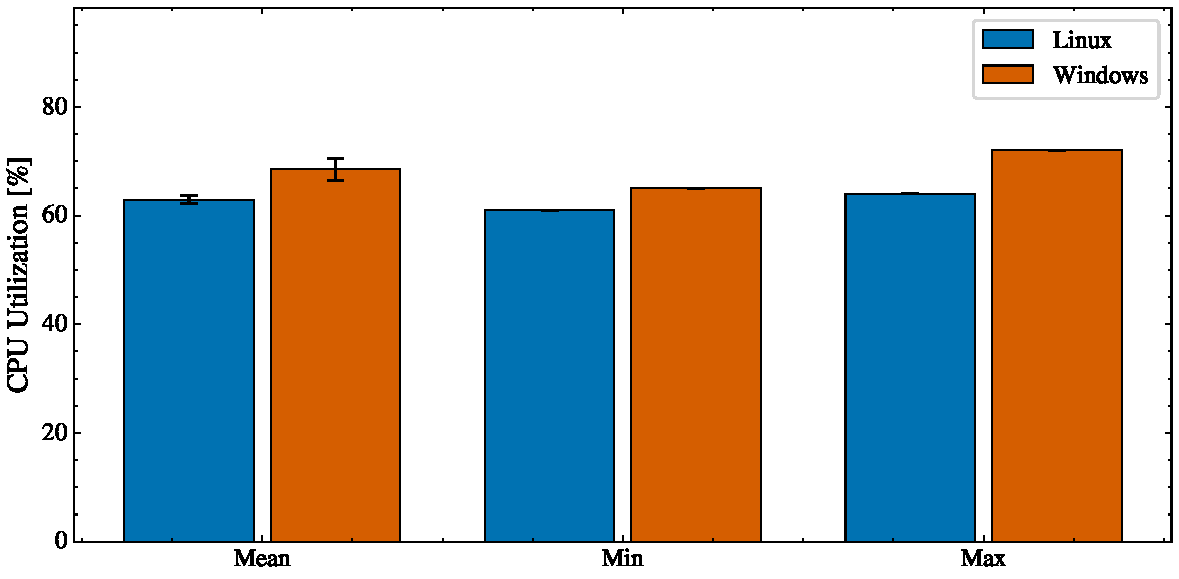
\includegraphics[width=\textwidth]{Messungen/OLD_10T/cpu_bars_combined.pdf}
\caption{Referenz, zehn Threads: CPU-Utilization}
\label{fig:4ref-10t-cpu}
\end{figure}

\section{First-In, First-Out}

In diesem Abschnitt werden die Ergebnisse der Messungen mit dem FIFO-Scheduler vorgestellt und mit der Referenz verglichen.
Für den FIFO-Scheduler wurden 2 verschiedene Warteschlangenlängen (50 und 500) getestet, 
um die Auswirkungen der Warteschlangenlänge auf die Performance zu untersuchen.
Im Unterschied zur Referenz wurden hier auch die internen Metriken wie Queue Time, 
Execution Time und der Anteil der synchronen Tasks erhoben.
Daher wird dieser Scheduler als Baseline für die Bewertung der anderen Scheduler herangezogen.

\begin{table}[H]
\caption{FIFO\_50: Laufzeit-, CPU- und RAM-Metriken (Mittelwerte $\pm$ Standardabweichung aus $n=20$ Läufen)}
\label{tab:fifo50-uebersicht-system}
\centering
\begingroup
\setlength{\tabcolsep}{4pt}
\resizebox{\textwidth}{!}{%
\begin{tabular}{@{}llllll@{}}
\toprule
Threads & OS & Runtime [s] & CPU [\%] & RAM Mittel [MB] & RAM Max [MB] \\
\midrule
1 & Linux   & 656 $\pm$ 3.15 & 23.6 $\pm$ 0.497 & 1065 $\pm$ 33.8 & 1705 \\
4 & Linux   & 271 $\pm$ 3.09 & 54.0 $\pm$ 0.447 & 1603 $\pm$ 22.7 & 2891 \\
10 & Linux  & 220 $\pm$ 3.34 & 62.2 $\pm$ 1.09 & 1954 $\pm$ 29.7 & 3968 \\
1 & Windows & 2506 $\pm$ 8.22 & 21.0 $\pm$ 0 & 1393 $\pm$ 6.47 & 6015 \\
4 & Windows & 1126 $\pm$ 23.3 & 48.6 $\pm$ 0.917 & 2188 $\pm$ 85.1 & 7766 \\
10 & Windows & 751 $\pm$ 25.4 & 71.1 $\pm$ 2.43 & 3213 $\pm$ 282 & 11672 \\
\bottomrule
\end{tabular}%
}
\endgroup
\end{table}

\begin{table}[H]
\caption{FIFO\_500: Laufzeit-, CPU- und RAM-Metriken (Mittelwerte $\pm$ Standardabweichung aus $n=20$ Läufen)}
\label{tab:fifo500-uebersicht-system}
\centering
\begingroup
\setlength{\tabcolsep}{4pt}
\resizebox{\textwidth}{!}{%
\begin{tabular}{@{}llllll@{}}
\toprule
Threads & OS & Runtime [s] & CPU [\%] & RAM Mittel [MB] & RAM Max [MB] \\
\midrule
1 & Linux   & 655 $\pm$ 3.82 & 23.7 $\pm$ 0.458 & 1057 $\pm$ 20.3 & 1630 \\
4 & Linux   & 274 $\pm$ 4.04 & 54.3 $\pm$ 0.843 & 1607 $\pm$ 30 & 3013 \\
10 & Linux  & 216 $\pm$ 3.34 & 63.8 $\pm$ 0.942 & 1922 $\pm$ 36.9 & 3649 \\
1 & Windows & 2502 $\pm$ 11.5 & 21.0 $\pm$ 0 & 1396 $\pm$ 4.84 & 6041 \\
4 & Windows & 1112 $\pm$ 29.2 & 49.9 $\pm$ 1.18 & 2294 $\pm$ 237 & 10782 \\
10 & Windows & 740 $\pm$ 31.5 & 72.2 $\pm$ 2.72 & 3107 $\pm$ 160 & 10672 \\
\bottomrule
\end{tabular}%
}
\endgroup
\end{table}

\noindent Wie wir in den Tabellen \ref{tab:fifo50-uebersicht-system} und \ref{tab:fifo500-uebersicht-system} sehen können,
sind die Laufzeiten, CPU-Auslastung und RAM-Auslastung für beide FIFO-Konfigurationen sehr ähnlich.
Bei der FIFO\_500 Konfiguration ist bei Windows bei vier Threads die maximale RAM-Auslastung mit 10782 MB deutlich höher 
als bei der FIFO\_50 Konfiguration mit 7766 MB,
was auf eine höhere Speichernutzung durch die längere Warteschlange hindeuten könnte.

\vspace{7.56mm}

\noindent Die Laufzeiten sind im Vergleich zur Referenz (Tabelle \ref{tab:old-scheduler-uebersicht}) 
auf Windows bei vier Threads um 7,20\% und bei zehn Threads um 9,10\% kürzer, während sie bei Linux nahezu identisch sind.

\begin{table}[H]
\caption{FIFO\_50: Runtime CV und Task-Metriken (Mittelwerte $\pm$ Standardabweichung aus $n=20$ Läufen)}
\label{tab:fifo50-uebersicht-task}
\centering
\begingroup
\setlength{\tabcolsep}{4pt}
\resizebox{\textwidth}{!}{%
\begin{tabular}{@{}llllll@{}}
\toprule
Threads & OS & Runtime CV [\%] & Queue [ms] & Exec [ms] & Sync Tasks [\%] \\
\midrule
1 & Linux   & 0.48 & 23.52 $\pm$ 0.12 & 0.98 $\pm$ 0.01 & 99.97 $\pm$ 0.00 \\
4 & Linux   & 1.14 & 27.98 $\pm$ 0.44 & 0.66 $\pm$ 0.01 & 54.06 $\pm$ 1.96 \\
10 & Linux  & 1.52 & 44.08 $\pm$ 1.49 & 1.08 $\pm$ 0.02 & 41.47 $\pm$ 2.06 \\
1 & Windows & 0.33 & 34.68 $\pm$ 0.12 & 1.09 $\pm$ 0.00 & 99.98 $\pm$ 0.00 \\
4 & Windows & 2.07 & 46.89 $\pm$ 1.04 & 1.09 $\pm$ 0.02 & 63.84 $\pm$ 5.46 \\
10 & Windows & 3.38 & 51.67 $\pm$ 2.22 & 1.43 $\pm$ 0.03 & 58.78 $\pm$ 4.66 \\
\bottomrule
\end{tabular}%
}
\endgroup
\end{table}



\begin{table}[H]
\caption{FIFO\_500: Runtime CV und Task-Metriken (Mittelwerte $\pm$ Standardabweichung aus $n=20$ Läufen)}
\label{tab:fifo500-uebersicht-task}
\centering
\begingroup
\setlength{\tabcolsep}{4pt}
\resizebox{\textwidth}{!}{%
\begin{tabular}{@{}llllll@{}}
\toprule
Threads & OS & Runtime CV [\%] & Queue [ms] & Exec [ms] & Sync Tasks [\%] \\
\midrule
1 & Linux   & 0.58 & 228.61 $\pm$ 1.51 & 0.97 $\pm$ 0.01 & 99.85 $\pm$ 0.00 \\
4 & Linux   & 1.48 & 278.90 $\pm$ 8.87 & 0.69 $\pm$ 0.01 & 65.44 $\pm$ 0.97 \\
10 & Linux  & 1.55 & 426.67 $\pm$ 10.08 & 1.10 $\pm$ 0.02 & 53.57 $\pm$ 2.30 \\
1 & Windows & 0.46 & 337.52 $\pm$ 1.60 & 1.09 $\pm$ 0.01 & 99.88 $\pm$ 0.00 \\
4 & Windows & 2.62 & 481.52 $\pm$ 13.97 & 1.10 $\pm$ 0.02 & 79.56 $\pm$ 2.98 \\
10 & Windows & 4.26 & 510.97 $\pm$ 17.40 & 1.43 $\pm$ 0.02 & 71.92 $\pm$ 3.80 \\
\bottomrule
\end{tabular}%
}
\endgroup
\end{table}

\noindent Die Anzahl an synchron ausgeführten Tasks ist bei beiden FIFO\_50 Konfigurationen geringer als bei der FIFO\_500 Konfiguration, 
wie in Tabelle \ref{tab:fifo50-uebersicht-task} und \ref{tab:fifo500-uebersicht-task} zu sehen ist.
Hier sieht man auch, dass die Queue Time bei der FIFO\_500 Konfiguration höher ist als bei der FIFO\_50 Konfiguration ist.

\subsection{Diskussion der FIFO-Ergebnisse}
\paragraph{Stabilität}
Wie beim Referenz-Scheduler zu beobachten ist, ist die CPU-Auslastung bei einem Thread über die Testläufe hinweg konstant,
was auf ein stabiles Testsystem hindeutet, siehe Abbildung \ref{fig:fifo50-1t-runtime}.
Auch bei vier Threads ist die CPU-Auslastung relativ stabil (Abbildung \ref{fig:fifo50-4t-runtime}), 
während bei zehn Threads (Abbildung \ref{fig:fifo50-10t-runtime}) eine größere Varianz in der CPU-Auslastung zu beobachten ist.
Selbiges spiegelt sich auch in den Laufzeiten wider, die mit zu-
nehmender Thread-Anzahl variabler werden, wie der Anstieg des Variationskoeffizienten 
in den Tabellen \ref{tab:fifo50-uebersicht-system} und \ref{tab:fifo500-uebersicht-system} zeigt.
Die ist vermutlich darauf zurückzuführen, dass die Anzahl der Threads die Anzahl an für das Testsystem bereit gestellten Kernen übersteigt, 
was zu einer höheren Konkurrenz um Ressourcen führt und damit zu einer höheren Varianz in der Performance.

\paragraph{Laufzeit}
Die bessere Performance im Bezug auf die Laufzeit des FIFO-Schedulers auf Windows bei mehreren Threads 
im Vergleich zur Referenz könnte zum Teil auf die asynchrone Task-Ausführung 
zum Ende einer Moduliteration zurückzuführen sein, bei welcher die Referenz noch auf synchron ausgeführte Objekte warten muss.
Diese Verbesserung ist auf Linux nicht zu beobachten.
Ein möglicher Grund könnte sein, dass die Module auf Linux weniger große Objekte erstellen, 
so dass der Vorteil der taskbasierten Ausführung nicht so stark zum Tragen kommt 
wie auf Windows, wo möglicherweise größere Objekte erstellt werden, die von der asynchronen Ausführung profitieren.
Hier sind weitere Untersuchungen notwendig,
um die genauen Gründe für die Unterschiede zwischen den Betriebssystemen zu verstehen.

\paragraph{Waiting Time und Burst Time}
Die Auswirkung der Warteschlangenlänge auf die Queue Time ist deutlich bei der FIFO\_500 Konfiguration im Vergleich zur FIFO\_50 Konfiguration zu sehen.
Mehr Tasks müssen in der Warteschlange warten, bevor sie ausgeführt werden können, was zu einer höheren Wartezeit führt.
Die übrigen Metriken deuten darauf hin, dass man die Warteschlangenlänge noch weiter reduzieren könnte, ohne die weiteren Metriken zu beeinträchtigen.
Mit weiteren Tests zur Warteschlangenlänge könnte die optimale Länge ermittelt werden, 
um die Performance der Wartezeit von Tasks zu verbessern, möglichst ohne die Performance der anderen Metriken zu beeinträchtigen.

\paragraph{Synchron ausgeführte Tasks und RAM-Auslastung}
Bei der FIFO\_500 Konfiguration ist der Anteil synchron ausgeführter Tasks deutlich höher 
als bei FIFO\_50.
Das deutet darauf hin, dass die längere Warteschlange mehr Tasks erzeugt,
die schließlich synchron ausgeführt werden müssen.
Auch die höhere maximale RAM-Auslastung der FIFO\_500 Konfiguration bei vier Threads gegenüber FIFO\_50 
kann mit der größeren Warteschlange zusammenhängen,
da mehr Tasks gleichzeitig vorgehalten werden und damit mehr Speicher belegen.

\paragraph{Vorteile und Nachteile der FIFO-Scheduler im Vergleich zur Referenz}
\begin{itemize}
    \item Vorteile:
    \begin{itemize}
        \item Auf Windows sind die Laufzeiten bei vier und zehn Threads gegenüber der Referenz deutlich kürzer.
        \item Die FIFO\_50-Konfiguration zeigt geringere Queue Time und geringere RAM-Spitzen als FIFO\_500.
    \end{itemize}
    \item Nachteile:
    \begin{itemize}
        \item Bei Linux ist kein klarer Laufzeitvorteil gegenüber der Referenz erkennbar.
        \item FIFO\_500 verursacht deutlich höhere Queue Time und höhere RAM-Maximalwerte, insbesondere auf Windows.
        \item Bei höherer Threadanzahl steigt die Varianz, was auf stärkere Ressourcenkonkurrenz hinweist.
    \end{itemize}
\end{itemize}

\section{Shortest-Subtree-Time-First}

\noindent In diesem Abschnitt werden die Ergebnisse der Messungen mit dem SSTF-Scheduler vorgestellt.
Das Ziel dieser Implementierung war es, die Anzahl der synchron ausgeführten Tasks zu reduzieren
und die Wartezeit von Tasks zu verbessern, indem die Tasks mit der kürzesten erwarteten Ausführungszeit zuerst ausgeführt werden.
Der SSTF-Scheduler wird mit den FIFO-Schedulern verglichen, um die Auswirkungen des Priorisierungsansatzes auf die Performance zu bewerten.

\begin{table}[H]
\caption{SSTF: Laufzeit-, CPU- und RAM-Metriken (Mittelwerte $\pm$ Standardabweichung aus $n=20$ Läufen)}
\label{tab:sstf-uebersicht-system}
\centering
\begingroup
\setlength{\tabcolsep}{4pt}
\resizebox{\textwidth}{!}{%
\begin{tabular}{@{}llllll@{}}
\toprule
Threads & OS & Runtime [s] & CPU [\%] & RAM Mittel [MB] & RAM Max [MB] \\
\midrule
1 & Linux   & 658 $\pm$ 3.27 & 23.9 $\pm$ 0.357 & 1068 $\pm$ 25.8 & 1688 \\
4 & Linux   & 273 $\pm$ 3.5 & 53.9 $\pm$ 0.436 & 1595 $\pm$ 36.4 & 3136 \\
10 & Linux  & 223 $\pm$ 4.11 & 62.3 $\pm$ 0.781 & 1922 $\pm$ 48.4 & 3631 \\
1 & Windows & 2526 $\pm$ 12.1 & 21.0 $\pm$ 0 & 1393 $\pm$ 5.3 & 5999 \\
4 & Windows & 1124 $\pm$ 24.4 & 48.9 $\pm$ 1.11 & 2209 $\pm$ 60.6 & 7844 \\
10 & Windows & 752 $\pm$ 25.6 & 71.8 $\pm$ 2.41 & 3210 $\pm$ 210 & 9592 \\
\bottomrule
\end{tabular}%
}
\endgroup
\end{table}

\noindent Tabelle \ref{tab:sstf-uebersicht-system} zeigt Laufzeit, CPU-Auslastung und RAM-Auslastung des SSTF-Schedulers.
Insgesamt liegen die Werte nahe bei den FIFO-Ergebnissen, unterscheiden sich aber in einzelnen Lastfällen.
Auffällig ist insbesondere, dass die maximale RAM-Auslastung bei zehn Threads auf Windows klar unter beiden FIFO-Konfigurationen liegt.


\begin{table}[H]
\caption{SSTF: Runtime CV und Task-Metriken (Mittelwerte $\pm$ Standardabweichung aus $n=20$ Läufen)}
\label{tab:sstf-uebersicht-task}
\centering
\begingroup
\setlength{\tabcolsep}{4pt}
\resizebox{\textwidth}{!}{%
\begin{tabular}{@{}llllll@{}}
\toprule
Threads & OS & Runtime CV [\%] & Queue [ms] & Exec [ms] & Sync Tasks [\%] \\
\midrule
1 & Linux   & 0.50 & 23.52 $\pm$ 0.12 & 0.49 $\pm$ 0.00 & 99.97 $\pm$ 0.00 \\
4 & Linux   & 1.28 & 25.71 $\pm$ 0.45 & 0.64 $\pm$ 0.01 & 44.09 $\pm$ 2.44 \\
10 & Linux  & 1.84 & 42.87 $\pm$ 1.04 & 1.08 $\pm$ 0.02 & 31.23 $\pm$ 1.16 \\
1 & Windows & 0.48 & 34.64 $\pm$ 0.18 & 0.70 $\pm$ 0.00 & 99.95 $\pm$ 0.00 \\
4 & Windows & 2.17 & 45.06 $\pm$ 1.34 & 1.07 $\pm$ 0.02 & 53.51 $\pm$ 4.05 \\
10 & Windows & 3.40 & 49.73 $\pm$ 1.61 & 1.44 $\pm$ 0.02 & 40.08 $\pm$ 2.65 \\
\bottomrule
\end{tabular}%
}
\endgroup
\end{table}

\noindent Tabelle \ref{tab:sstf-uebersicht-task} enthält Runtime CV, Queue Time, Execution Time und den Anteil synchroner Tasks.
Die Runtime CV bleibt im Bereich der FIFO-Werte, zeigt aber leichte Abweichungen je nach Last.
Gleichzeitig fällt die Queue Time gegenüber FIFO\_50 und FIFO\_500 etwas geringer aus.
Besonders deutlich ist die niedrigere Execution Time im Vergleich zu beiden FIFO-Varianten.
Zusätzlich sinkt der Anteil synchron ausgeführter Tasks gegenüber beiden FIFO-Konfigurationen klar.

\subsection{Diskussion der SSTF-Ergebnisse}

\paragraph{Stabilität}
Die Stabilität ist insgesamt vergleichbar mit den FIFO-Schedulern:
Bei einem Thread bleibt die CPU-Auslastung über die Testläufe hinweg konstant,
während mit steigender Thread-Anzahl die Varianz zunimmt (siehe Abbildung \ref{fig:sstf-1t-runtime}, \ref{fig:sstf-4t-runtime} und \ref{fig:sstf-10t-runtime}).

\paragraph{Laufzeit}
Die Laufzeiten des SSTF-Schedulers liegen nahe an den FIFO-Werten;
die Unterschiede bleiben insgesamt gering und hängen vom jeweiligen Lastfall ab.

\paragraph{Waiting Time und Burst Time}
Im Vergleich zu beiden FIFO-Konfigurationen fällt die Queue Time bei SSTF etwas geringer aus.
Das spricht dafür, dass die Priorisierung kürzerer Tasks die Wartezeit verbessert.
Der Grund hierfür muss noch weiter untersucht werden.

\paragraph{Synchron ausgeführte Tasks und RAM-Auslastung}
Bei SSTF ist der Anteil synchron ausgeführter Tasks gegenüber beiden FIFO-Konfigurationen deutlich geringer.
Damit spricht Vieles dafür, dass die Priorisierung kürzerer Tasks die notwendige Synchronisation reduziert.
Hinzu kommt die niedrigere maximale RAM-Auslastung bei zehn Threads auf Windows im Vergleich zu beiden FIFO-Varianten.
Insgesamt lassen sich hier deutliche Verbesserungen gegenüber den FIFO-Schedulern feststellen.

\paragraph{Vorteile und Nachteile im Vergleich zu FIFO}
\begin{itemize}
    \item Vorteile:
    \begin{itemize}
        \item Geringere Queue Time als bei beiden FIFO-Konfigurationen, besonders unter Last.
        \item Deutlich geringerer Anteil synchron ausgeführter Tasks bei vier und zehn Threads.
        \item Niedrigere RAM-Maximalwerte auf Windows bei zehn Threads im Vergleich zu FIFO\_50 und FIFO\_500.
    \end{itemize}
    \item Nachteile:
    \begin{itemize}
        \item Kein durchgängiger Laufzeitvorteil gegenüber FIFO, Unterschiede sind je nach Betriebssystem und Threadzahl gering.
        \item Bei hoher Last steigt die Runtime CV ebenfalls an und bleibt damit sensitiv gegenüber Lastspitzen.
        \item Der Nutzen hängt von der Qualität der Priorisierung ab, bei abweichender Laststruktur kann der Vorteil geringer ausfallen.
    \end{itemize}
\end{itemize}

\section{Work-Stealing mit SSTF-Priorisierung}
Hier werden die Ergebnisse der Messungen des Work-Stealing-Schedulers mit SSTF-Priorisierung vorgestellt.
Das Ziel dieser Implementierung war es, die Vorteile des SSTF-Schedulers mit der Flexibilität und Lastverteilung des Work-Stealing-Ansatzes zu kombinieren und Lock-Contention zu reduzieren.
Der Work-Stealing Scheduler mit SSTF-Priorisierung wird primär mit dem SSTF-Scheduler verglichen, 
um die Auswirkungen des Work-Stealing-Ansatzes auf die Performance zu bewerten, 
da beide Scheduler die gleiche Priorisierungsstrategie verwenden.

\begin{table}[H]
\caption{WS: Laufzeit-, CPU- und RAM-Metriken (Mittelwerte $\pm$ Standardabweichung aus $n=20$ Läufen)}
\label{tab:ws-uebersicht-system}
\centering
\begingroup
\setlength{\tabcolsep}{4pt}
\resizebox{\textwidth}{!}{%
\begin{tabular}{@{}llllll@{}}
\toprule
Threads & OS & Runtime [s] & CPU [\%] & RAM Mittel [MB] & RAM Max [MB] \\
\midrule
1 & Linux   & 660 $\pm$ 3.47 & 23.5 $\pm$ 0.5 & 1065 $\pm$ 17.6 & 1653 \\
4 & Linux   & 294 $\pm$ 3.93 & 51.2 $\pm$ 0.927 & 1528 $\pm$ 31.7 & 2573 \\
10 & Linux  & 220 $\pm$ 3.16 & 63.2 $\pm$ 0.829 & 1868 $\pm$ 47.7 & 3751 \\
1 & Windows & 2526 $\pm$ 10.2 & 21.0 $\pm$ 0 & 1389 $\pm$ 6.46 & 5991 \\
4 & Windows & 1145 $\pm$ 34.6 & 47.8 $\pm$ 1.26 & 2087 $\pm$ 54 & 7648 \\
10 & Windows & 747 $\pm$ 34.2 & 71.9 $\pm$ 3.37 & 2904 $\pm$ 243 & 11457 \\
\bottomrule
\end{tabular}%
}
\endgroup
\end{table}

\noindent In Tabelle \ref{tab:ws-uebersicht-system} sind die Laufzeit, CPU-Auslastung und RAM-Auslastung für den Work-Stealing mit SSTF-Priorisierung aufgelistet.
Die Werte liegen insgesamt nahe am SSTF-Scheduler, unterscheiden sich jedoch in einzelnen Punkten.
So ist die mittlere RAM-Utilization durchgehend niedriger als bei SSTF, während die maximale RAM-Auslastung bei zehn Threads auf Windows höher ausfällt.

\begin{table}[H]
\caption{WS: Runtime CV und Task-Metriken (Mittelwerte $\pm$ Standardabweichung aus $n=20$ Läufen)}
\label{tab:ws-uebersicht-task}
\centering
\begingroup
\setlength{\tabcolsep}{4pt}
\resizebox{\textwidth}{!}{%
\begin{tabular}{@{}llllll@{}}
\toprule
Threads & OS & Runtime CV [\%] & Queue [ms] & Exec [ms] & Sync Tasks [\%] \\
\midrule
1 & Linux   & 0.53 & 46.26 $\pm$ 0.28 & 0.98 $\pm$ 0.01 & 99.95 $\pm$ 0.00 \\
4 & Linux   & 1.33 & 58.52 $\pm$ 1.09 & 0.91 $\pm$ 0.01 & 80.61 $\pm$ 1.21 \\
10 & Linux  & 1.44 & 84.72 $\pm$ 1.28 & 1.10 $\pm$ 0.01 & 27.09 $\pm$ 1.63 \\
1 & Windows & 0.40 & 65.91 $\pm$ 0.40 & 1.09 $\pm$ 0.00 & 99.83 $\pm$ 0.00 \\
4 & Windows & 3.03 & 90.46 $\pm$ 2.76 & 1.11 $\pm$ 0.02 & 53.36 $\pm$ 4.64 \\
10 & Windows & 4.58 & 97.23 $\pm$ 3.15 & 1.44 $\pm$ 0.03 & 35.31 $\pm$ 3.25 \\
\bottomrule
\end{tabular}%
}
\endgroup
\end{table}

\noindent In Tabelle \ref{tab:ws-uebersicht-task} sind die Runtime CV, Queue Time, Execution Time und der Anteil der synchronen Tasks für den Work-Stealing mit SSTF-Priorisierung aufgelistet.
Die Runtime CV bewegt sich im Bereich der SSTF-Werte, zeigt aber in einzelnen Szenarien größere Ausschläge.
Im Vergleich zu beiden FIFO-Konfigurationen ist die Queue Time bei Work-Stealing mit SSTF-Priorisierung deutlich höher.
Auch der Anteil synchron ausgeführter Tasks schwankt stärker als bei SSTF.



\subsection{Diskussion der WS-Ergebnisse}

\paragraph{Stabilität}
Die Stabilität entspricht weitgehend dem Bild der FIFO-Scheduler und des SSTF-Schedulers.
Bei einem Thread bleibt die CPU-Auslastung über die Testläufe hinweg konstant,
mit steigender Thread-Anzahl nimmt die Varianz jedoch zu (siehe Abbildung \ref{fig:ws-1t-runtime}, \ref{fig:ws-4t-runtime} und \ref{fig:ws-10t-runtime}).

\paragraph{Laufzeit}
Die Laufzeiten von Work-Stealing mit SSTF-Priorisierung sind insgesamt nah an den SSTF-Werten,
weichen je nach Plattform und Lastfall aber leicht ab.

\paragraph{Waiting Time und Burst Time}
Im Vergleich zu beiden FIFO-Konfigurationen ist die Wartezeit der Tasks bei Work-Stealing mit SSTF-Priorisierung deutlich höher.
Eine angepasste Implementierung könnte diese Wartezeit reduzieren,
etwa durch eine Begrenzung der Warteschlangengröße pro Thread, damit Tasks nicht zu lange in den Queues verbleiben,
bevor sie ausgeführt werden.

\paragraph{Synchron ausgeführte Tasks und RAM-Auslastung}
Auffällig ist bei vier Threads die nahezu doppelt so hohe Zahl synchron ausgeführter Tasks gegenüber SSTF,
was auf Optimierungspotenzial in dieser Konfiguration hindeutet.
Ebenso spricht die höhere maximale RAM-Auslastung bei zehn Threads auf Windows gegenüber SSTF dafür,
dass die aktuelle Work-Stealing-Strategie mehr Tasks gleichzeitig in den Queues hält und dadurch mehr Speicher benötigt.
Gleichzeitig fällt die mittlere RAM-Auslastung über alle Konfigurationen hinweg niedriger aus,
was auf Vorteile bei der durchschnittlichen Speichernutzung schließen lässt.

\paragraph{Vorteile und Nachteile des Work-Stealing-Schedulers mit SSTF-Priorisierung im Vergleich zum SSTF-Scheduler}
\begin{itemize}
    \item Vorteile:
    \begin{itemize}
        \item In einigen Fällen könnte die Work-Stealing-Implementierung zu einer besseren Speichernutzung führen, wie die durchgehend niedrigere mittlere RAM-Auslastung im Vergleich zum SSTF-Scheduler zeigt.
    \end{itemize}
    \item Nachteile:
    \begin{itemize}
        \item Die Wartezeit der Tasks ist bei Work-Stealing mit SSTF-Priorisierung im Vergleich zu beiden FIFO-Konfigurationen deutlich höher.
        \item Die Anzahl der synchron ausgeführten Tasks schwankt im Vergleich zum SSTF-Scheduler, was auf eine nicht optimale Implementierung des Work-Stealing-Algorithmus hindeuten könnte.
        \item Die höhere maximale RAM-Auslastung bei zehn Threads auf Windows im Vergleich zum SSTF-Scheduler könnte ebenfalls auf die Work-Stealing-Implementierung zurückzuführen sein, da mehr Tasks in der Warteschlange gehalten werden müssen, was zu einem höheren Speicherbedarf führt.
    \end{itemize}
\end{itemize}


\section{Diskussion der Ergebnisse}

\noindent Die Ergebnisse der Messungen zeigen, dass die verschiedenen Scheduling-Algorithmen 
unterschiedliche Auswirkungen auf die Performance
von verschiedenen Metriken haben, wie Laufzeit, CPU-Auslastung, RAM-Auslastung, 
Wartezeit von Tasks und Anzahl der synchron ausgeführten Tasks.
Für die Nutzer des Scanners ist die Laufzeit von oberster Priorität, 
möglichst in Kombination mit einer geringer Ressourcen-Auslastung.
Ein Scanner mit responsivem Verhalten und entsprechend niedriger Wartezeit von Tasks, 
ist ebenfalls wünschenswert,sollte allerdings nicht auf Kosten einer höheren Laufzeit implementiert werden.
Die Anzahl der synchron ausgeführten Tasks sollte möglichst gering sein, um die Vorteile der taskbasierten Ausführung zu nutzen,
hat für den Nutzer allerdings keine direkte Auswirkung und somit eine niedrigere Priorität.

\vspace{7.56mm}
\noindent Die hier verwendeten Grafiken zeigen die Mittelwerte von jeweils 20 Messungen der Laufzeit, 
CPU-Auslastung und RAM-Auslastung der verschiedenen Scheduling-Algorithmen 
bei verschiedenen Thread-Anzahlen auf Windows und Linux.

\vspace{7.56mm}

\noindent Die Ergebnisse zeigen bei einem Thread keine revelanten Unterschiede zwischen den verschiedenen Scheduling-Algorithmen, siehe 
Abbildung \ref{fig:schedulercmp-1t-runtime}, \ref{fig:schedulercmp-1t-cpu} und \ref{fig:schedulercmp-1t-ram}.
Bei Singlethread-Ausführung zeigen alle Scheduler vergleichbare Performance. 
Dies ist erwartet, da Scheduling-Vorteile erst mit Parallelismus zum Tragen kommen.

\begin{figure}[H]
\centering
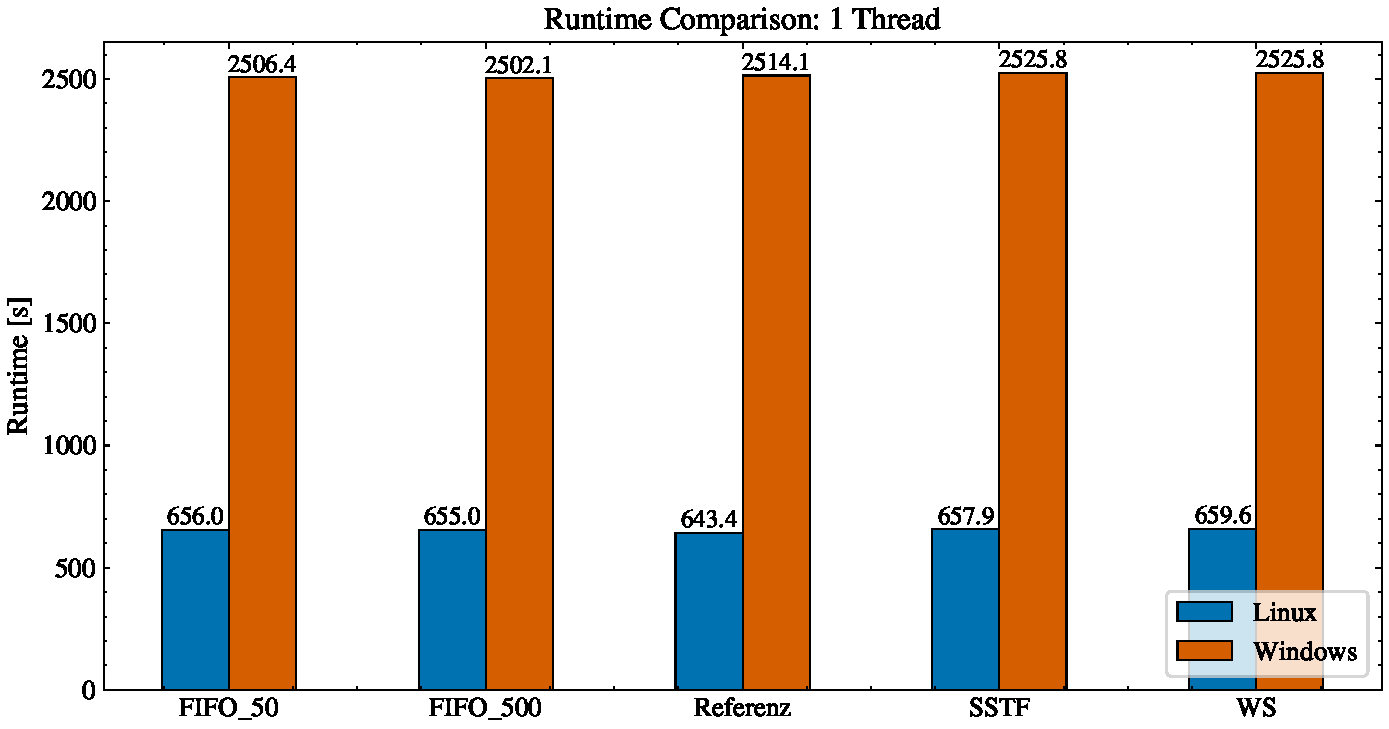
\includegraphics[width=\textwidth]{Messungen/Scheduler_Comparison/scheduler_1T_runtime.pdf}
\caption{Scheduler-Vergleich bei einem Thread: Runtime}
\label{fig:schedulercmp-1t-runtime}
\end{figure}

\begin{figure}[H]
\centering
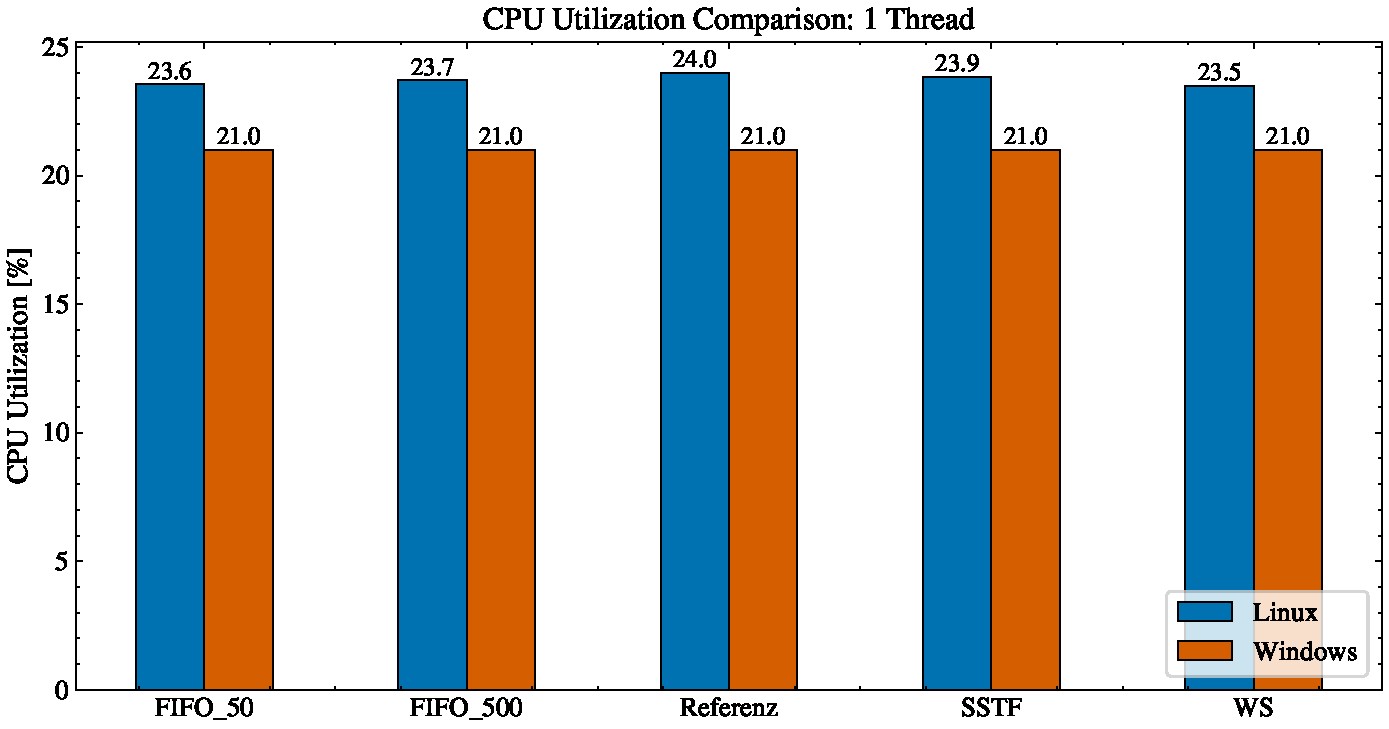
\includegraphics[width=\textwidth]{Messungen/Scheduler_Comparison/scheduler_1T_cpu.pdf}
\caption{Scheduler-Vergleich bei einem Thread: CPU-Utilization}
\label{fig:schedulercmp-1t-cpu}
\end{figure}

\begin{figure}[H]
\centering
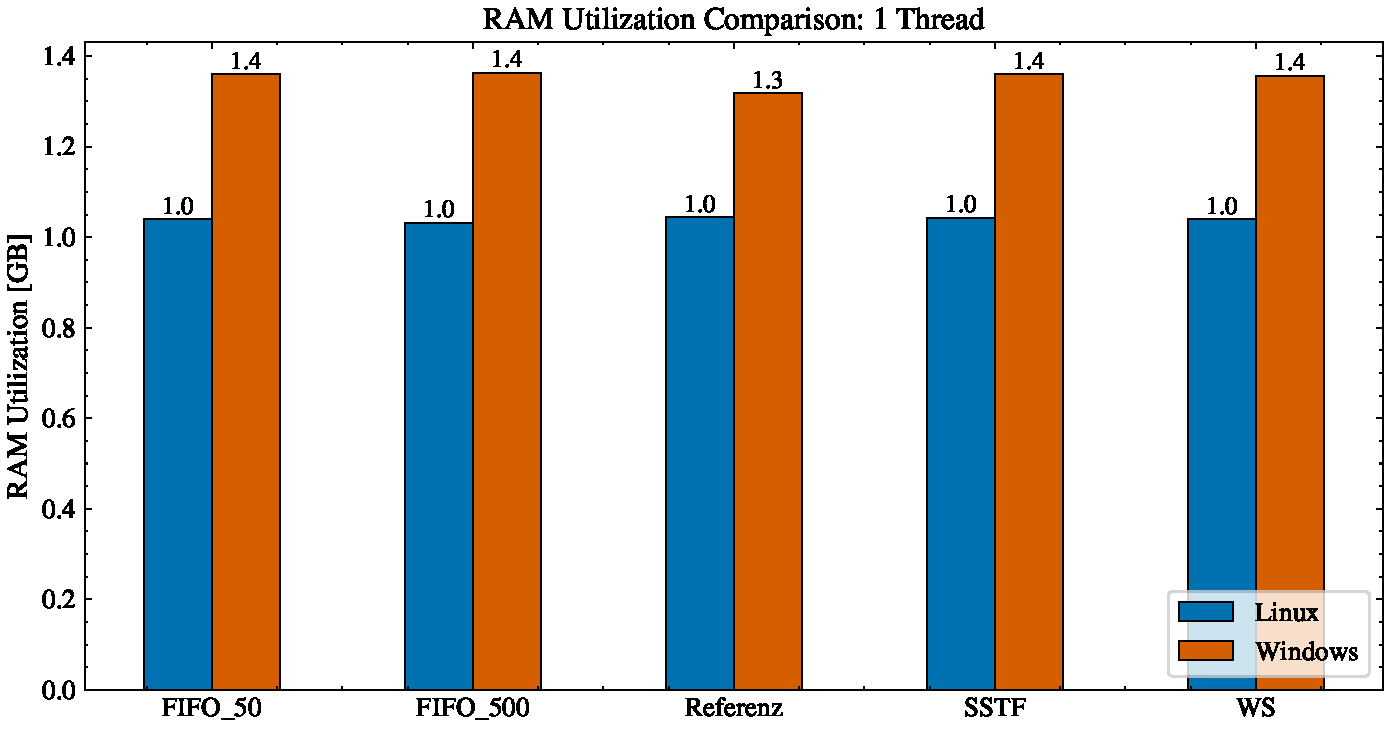
\includegraphics[width=\textwidth]{Messungen/Scheduler_Comparison/scheduler_1T_ram.pdf}
\caption{Scheduler-Vergleich bei einem Thread: RAM-Utilization}
\label{fig:schedulercmp-1t-ram}
\end{figure}

\noindent Erst bei der Verwendung von mehreren Threads werden Unterschiede zwischen den verschiedenen Scheduling-Algorithmen sichtbar.
Bei vier Threads ist der Unterschied in der Laufzeit auf Windows deutlich erkennbar, siehe Abbildung \ref{fig:schedulercmp-4t-runtime}.
Gegenüber der Referenz (1213.83 $\pm$ 26.95\,s) sind alle neuen Scheduler schneller:
FIFO\_50 mit 1126.42 $\pm$ 23.26\,s (-7.20\%), FIFO\_500 mit 1112.04 $\pm$ 29.19\,s (-8.39\%), SSTF mit 1123.66 $\pm$ 24.39\,s (-7.43\%) und Work-Stealing mit 1144.78 $\pm$ 34.65\,s (-5.69\%).
Auf Linux ist dieser Vorteil nicht in gleicher Form sichtbar, dort liegen die Laufzeiten deutlich näher beieinander.

\vspace{7.56mm}

\noindent Zwischen FIFO\_50, FIFO\_500 und SSTF sind Laufzeit und CPU-Auslastung bei vier Threads insgesamt ähnlich, siehe
Abbildung \ref{fig:schedulercmp-4t-runtime} und \ref{fig:schedulercmp-4t-cpu}.
Deutliche Unterschiede zeigen sich jedoch bei den internen Metriken:
FIFO\_500 hat mit 481.52 $\pm$ 13.97\,ms eine stark erhöhte Queue Time und mit 10782\,MB die höchste RAM-Spitze.
SSTF erreicht mit 45.06 $\pm$ 1.34\,ms die niedrigste Queue Time und reduziert den Anteil synchron ausgeführter Tasks auf 53.51\%
(FIFO\_50: 63.84\%, FIFO\_500: 79.56\%).
Work-Stealing liegt bei der Queue Time mit 90.46 $\pm$ 2.76\,ms deutlich höher, zeigt aber bei den synchronen Tasks mit 53.36\% einen ähnlichen Wert wie SSTF.

\vspace{7.56mm}

\noindent Nach den festgelegten Prioritäten (Laufzeit vor Ressourcenauslastung und Responsivität) ist bei vier Threads
SSTF die ausgewogenste Konfiguration:
vergleichbare Laufzeit zur schnelleren FIFO-Varianten, gleichzeitig geringere Queue Time und deutlich weniger synchron ausgeführte Tasks.

\begin{figure}[H]
\centering
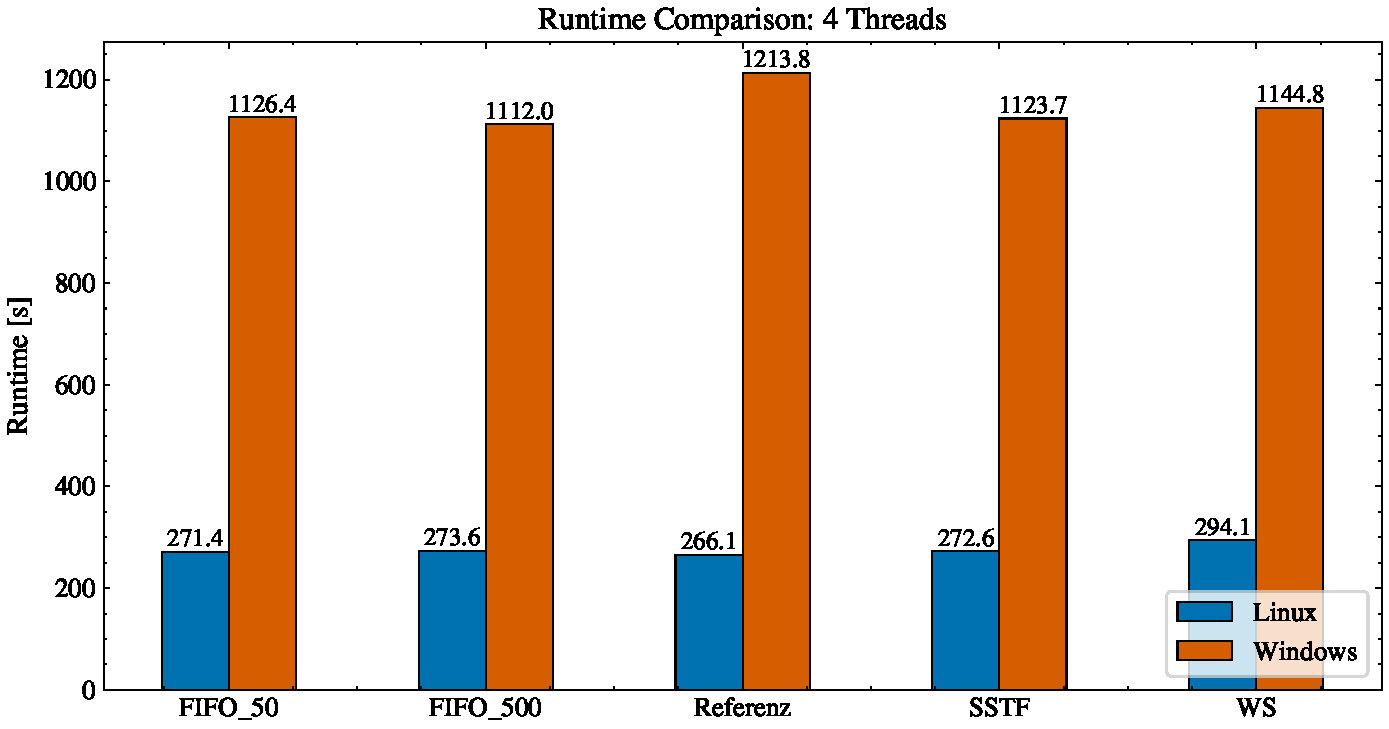
\includegraphics[width=\textwidth]{Messungen/Scheduler_Comparison/scheduler_4T_runtime.pdf}
\caption{Scheduler-Vergleich bei vier Threads: Runtime}
\label{fig:schedulercmp-4t-runtime}
\end{figure}

\begin{figure}[H]
\centering
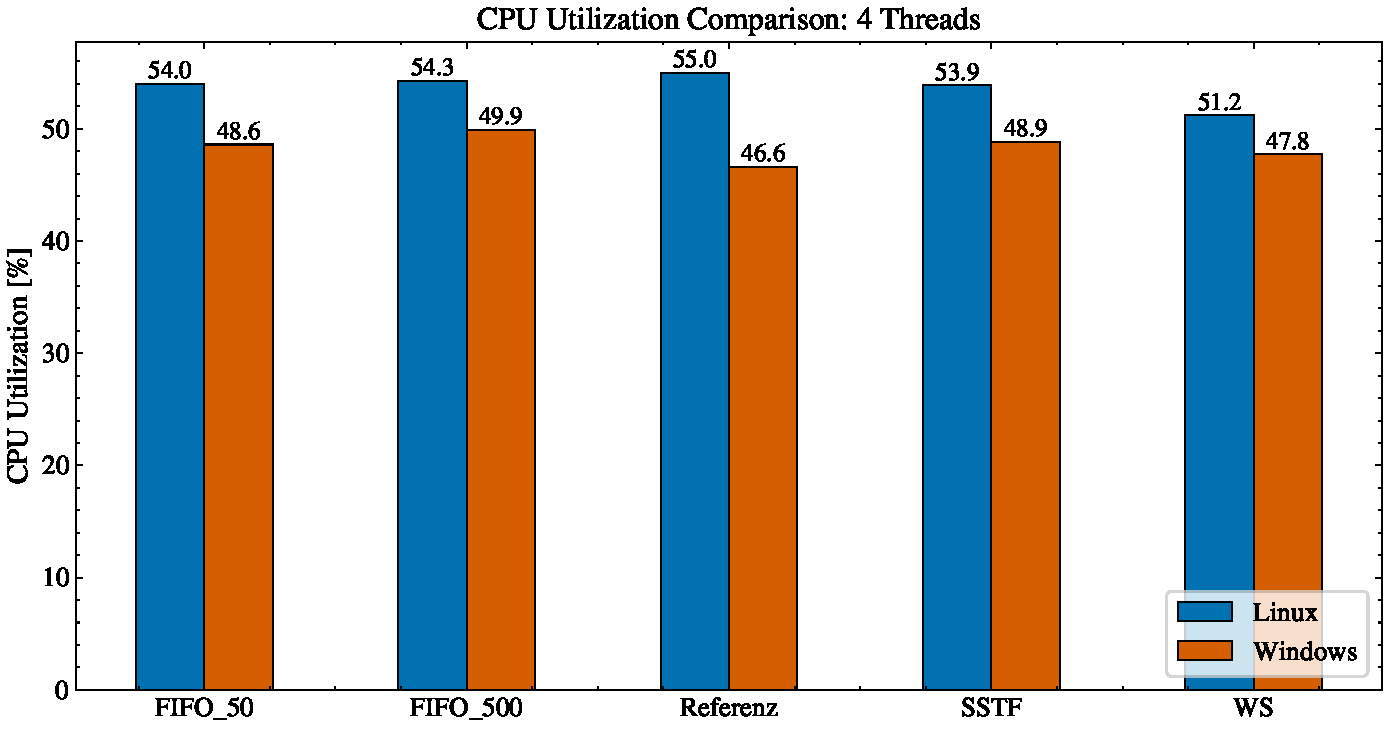
\includegraphics[width=\textwidth]{Messungen/Scheduler_Comparison/scheduler_4T_cpu.pdf}
\caption{Scheduler-Vergleich bei vier Threads: CPU-Utilization}
\label{fig:schedulercmp-4t-cpu}
\end{figure}

\begin{figure}[H]
\centering
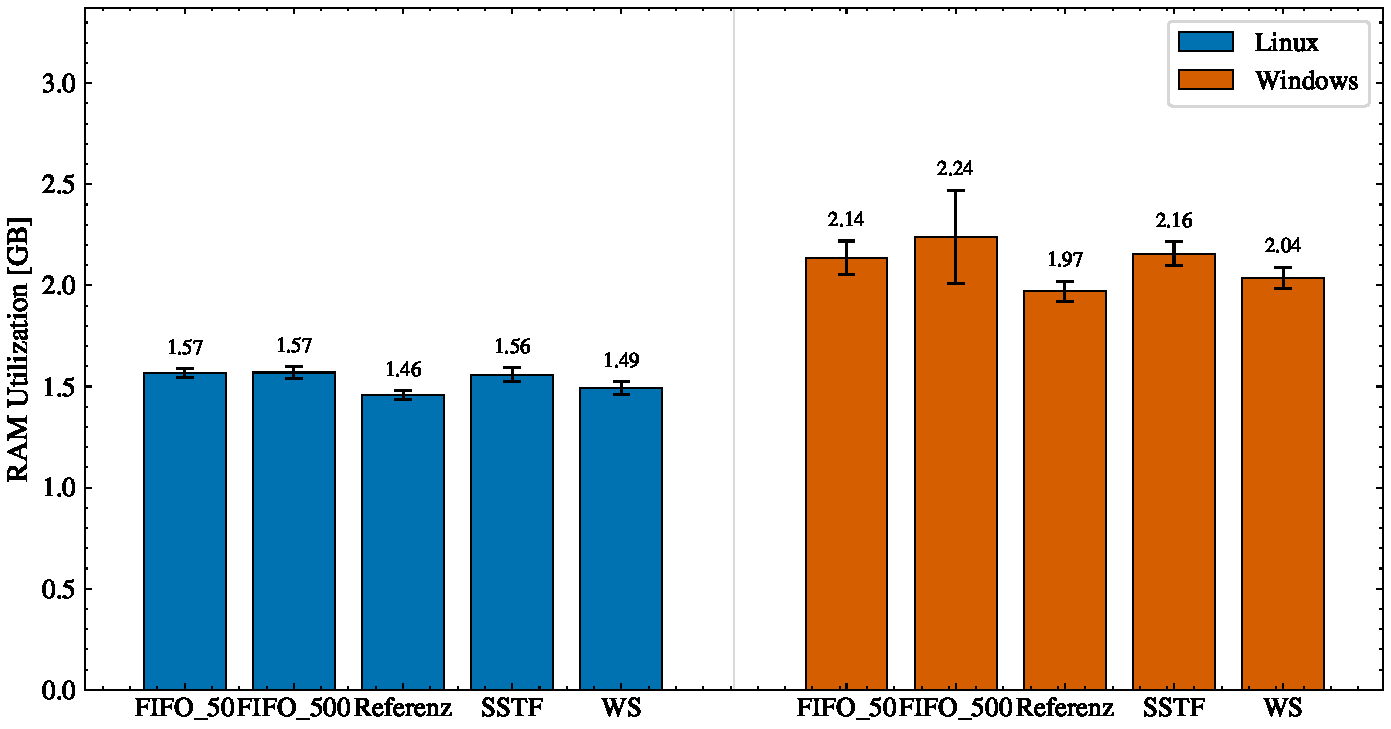
\includegraphics[width=\textwidth]{Messungen/Scheduler_Comparison/scheduler_4T_ram.pdf}
\caption{Scheduler-Vergleich bei vier Threads: RAM-Utilization}
\label{fig:schedulercmp-4t-ram}
\end{figure}

\noindent Bei zehn Threads werden die Unterschiede zwischen den Scheduling-Algorithmen noch deutlicher, siehe
Abbildung \ref{fig:schedulercmp-10t-runtime}, \ref{fig:schedulercmp-10t-cpu} und \ref{fig:schedulercmp-10t-ram}.
Auf Windows sind alle neuen Scheduler weiterhin klar schneller als die Referenz (825.78 $\pm$ 20.53\,s):
FIFO\_50 mit 750.65 $\pm$ 25.36\,s (-9.10\%), FIFO\_500 mit 740.05 $\pm$ 31.51\,s (-10.38\%), SSTF mit 752.41 $\pm$ 25.56\,s (-8.88\%) und Work-Stealing mit 747.43 $\pm$ 34.23\,s (-9.49\%).
Auf Linux liegen die Laufzeiten dagegen sehr nah beieinander, ein klarer Laufzeitvorteil eines einzelnen Schedulers ist dort nicht erkennbar.

\vspace{7.56mm}

\noindent Deutliche Unterschiede zeigen sich bei den internen Metriken und der Ressourcencharakteristik:
SSTF reduziert den Anteil synchron ausgeführter Tasks auf 40.08\% (FIFO\_50: 58.78\%, FIFO\_500: 71.92\%)
und erreicht damit eine klar bessere Task-Parallelisierung als beide FIFO-Varianten.
Work-Stealing senkt den Anteil synchroner Tasks weiter auf 35.31\% und erreicht
zugleich mit 747.43 $\pm$ 34.23\,s die beste Laufzeit auf Windows, knapp vor SSTF mit 752.41 $\pm$ 25.56\,s,
geht jedoch mit deutlich höherer Queue Time (97.23 $\pm$ 3.15\,ms) einher.
Bei der RAM-Spitze zeigt SSTF auf Windows mit 9592\,MB den besten Wert unter den neuen Schedulern,
während Work-Stealing mit 11457\,MB deutlich höher liegt.

\vspace{7.56mm}

\noindent Nach den festgelegten Prioritäten ist damit auch bei zehn Threads SSTF die robusteste Gesamtwahl:
nahezu beste Laufzeit, klar reduzierte Synchronisation und günstigeres RAM-Maximum.
Work-Stealing ist eine interessante Alternative für maximale Laufzeitoptimierung auf Windows,
erfordert aber weitere Optimierung der Queue Time und Speichercharakteristik.

\begin{figure}[H]
\centering
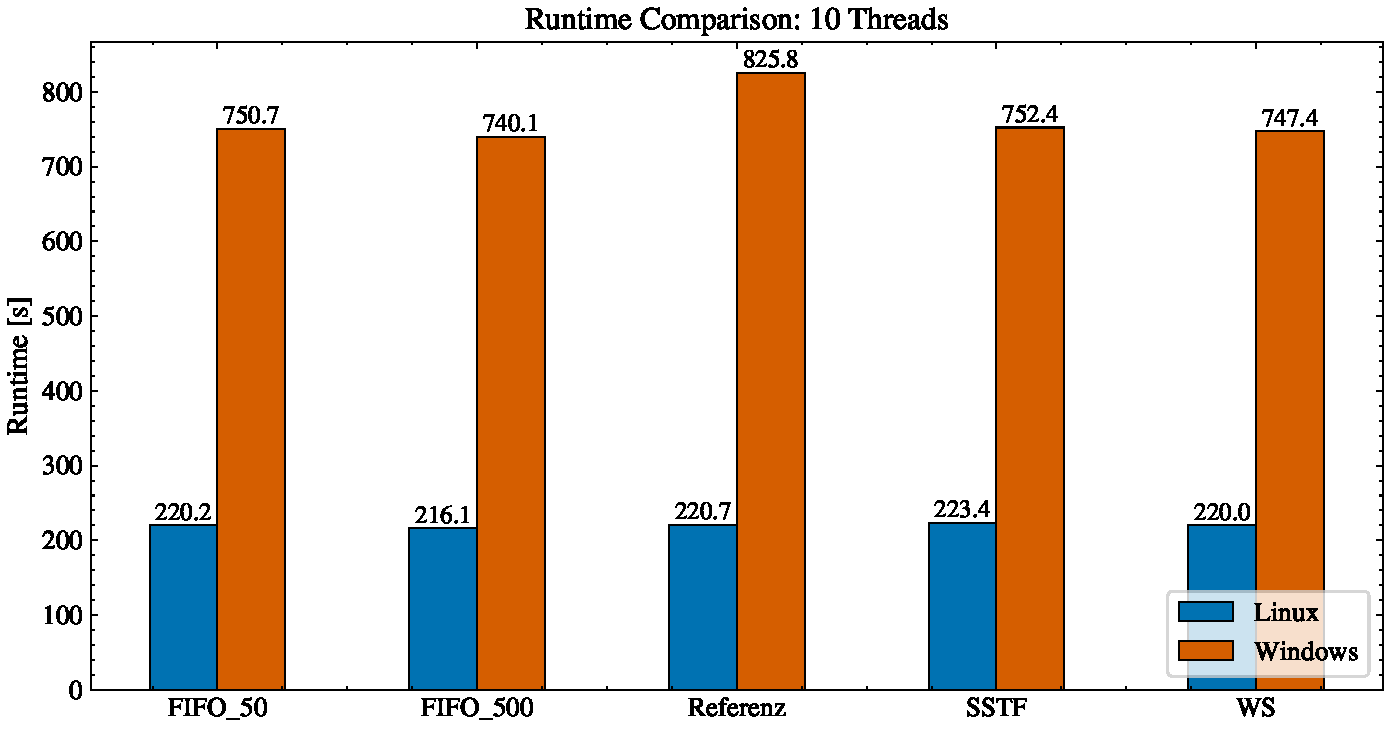
\includegraphics[width=\textwidth]{Messungen/Scheduler_Comparison/scheduler_10T_runtime.pdf}
\caption{Scheduler-Vergleich bei zehn Threads: Runtime}
\label{fig:schedulercmp-10t-runtime}
\end{figure}

\begin{figure}[H]
\centering
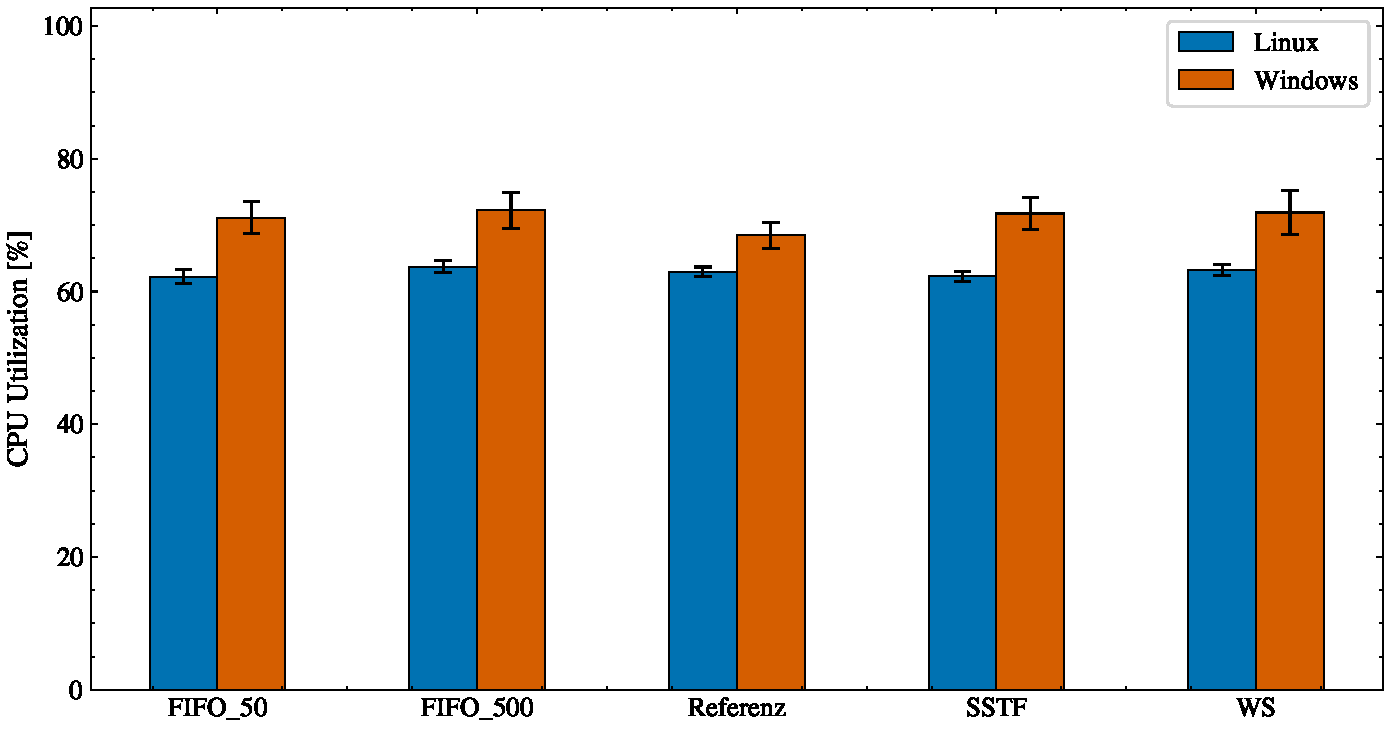
\includegraphics[width=\textwidth]{Messungen/Scheduler_Comparison/scheduler_10T_cpu.pdf}
\caption{Scheduler-Vergleich bei zehn Threads: CPU-Utilization}
\label{fig:schedulercmp-10t-cpu}
\end{figure}

\begin{figure}[H]
\centering
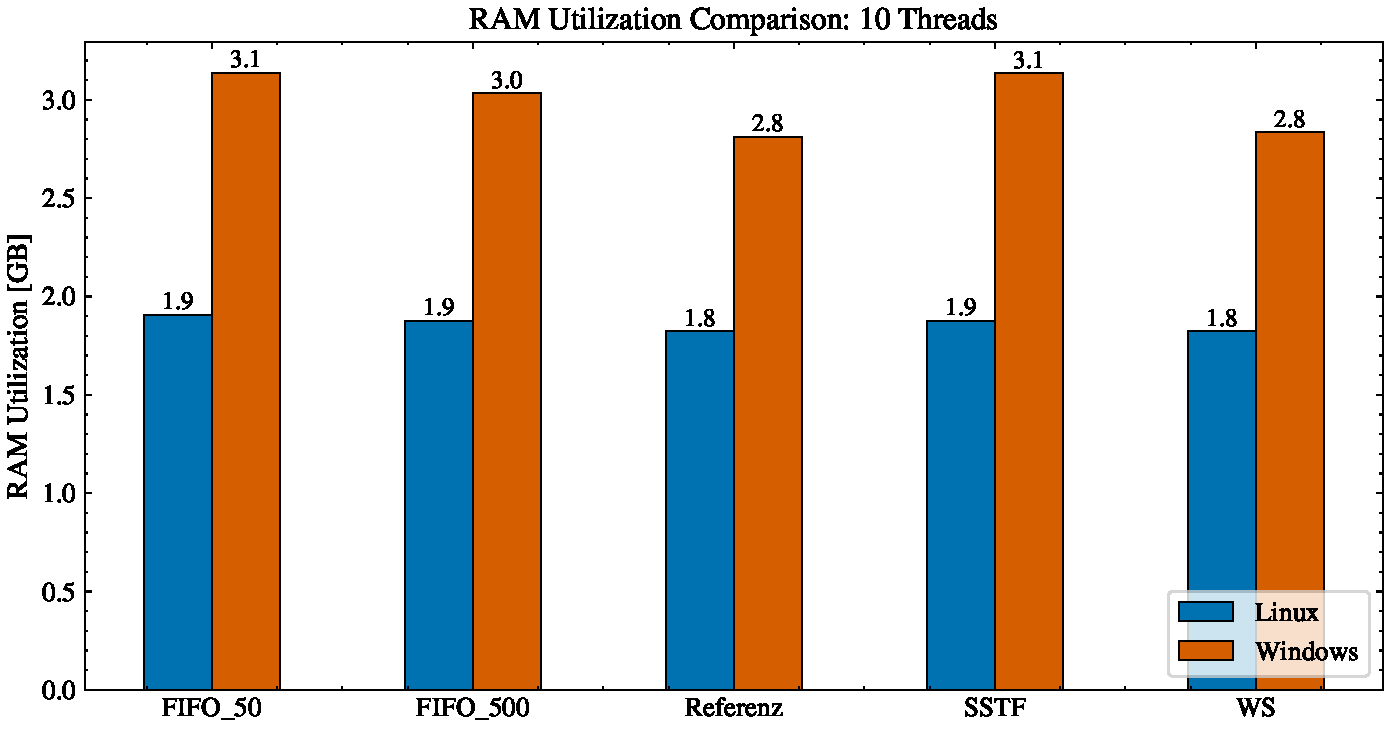
\includegraphics[width=\textwidth]{Messungen/Scheduler_Comparison/scheduler_10T_ram.pdf}
\caption{Scheduler-Vergleich bei zehn Threads: RAM-Utilization}
\label{fig:schedulercmp-10t-ram}
\end{figure}

\noindent Die Auswertung zeigt, dass SSTF im Bezug auf die gewählten Prioritäten die
beste Gesamtbalance aus Laufzeit, Stabilität und Ressourceneffizienz bietet
und damit als bevorzugte Scheduler-Strategie empfohlen werden kann.

\noindent Weitere Tests mit optimierten Implementierungen und auf verschiedenen Systemen sind jedoch empfehlenswert.

\end{sloppypar}
